\section{相关技术与理论}

\subsection{\TeX{} 排版系统概述}

\TeX{} 是由 Donald E. Knuth 于 1984 年开发的排版系统，其核心优势在于精确的版面控制与高质量的数学公式排版\cite{knuth1984texbook}。\TeX{} 采用标记语言描述文档结构，通过编译生成最终的版式文件（通常为 PDF）。

\subsection{常用宏包介绍}

表~\ref{tab:packages} 列出了本模板使用的主要宏包及其功能说明。

\begin{table}[htbp]
\centering
\caption{本模板使用的主要宏包}
\label{tab:packages}
\zihao{-5}\songti
\begin{tabular}{lll}
\toprule
序号 & 宏包名称 & 主要功能 \\
\midrule
1 & ctex & 中文支持、字体配置 \\
2 & geometry & 页面尺寸与页边距设置 \\
3 & titlesec / titletoc & 标题与目录格式定制 \\
4 & setspace & 行距控制 \\
5 & gbt7714 & 参考文献国标格式 \\
6 & hyperref & 超链接与 PDF 书签 \\
\bottomrule
\end{tabular}
\end{table}

\subsection{LaTeX 安装指南}

为了使用本模板，需要在计算机上安装 LaTeX 发行版。以下是不同操作系统的安装方法：

\subsubsection{Windows 系统}

1. **下载并安装 TeX Live**
   - 访问 \url{https://tug.org/texlive/}
   - 下载 `install-tl-windows.exe` 安装程序
   - 运行安装程序，选择完整安装（约 6GB 空间）
   - 安装完成后，重启电脑以更新环境变量

2. **验证安装**
   - 打开命令提示符（CMD）
   - 输入 `xelatex --version` 查看是否安装成功

\subsubsection{Mac 系统}

1. **下载并安装 MacTeX**
   - 访问 \url{https://tug.org/mactex/}
   - 下载最新版本的 MacTeX 安装包（约 4GB）
   - 运行安装程序，按照提示完成安装

2. **验证安装**
   - 打开终端（Terminal）
   - 输入 `xelatex --version` 查看是否安装成功


\subsection{公式与图表排版}

\LaTeX{} 的公式排版能力是其核心优势之一。行内公式如 $E=mc^2$ 可直接嵌入正文，独立编号公式则如式~(\ref{eq:quadratic}) 所示。

\begin{equation}
    x = \frac{-b \pm \sqrt{b^2 - 4ac}}{2a}
    \label{eq:quadratic}
\end{equation}

图~\ref{fig:latex-process} 展示了 \LaTeX{} 文档的基本编译流程。

\begin{figure}[htbp]
    \centering
    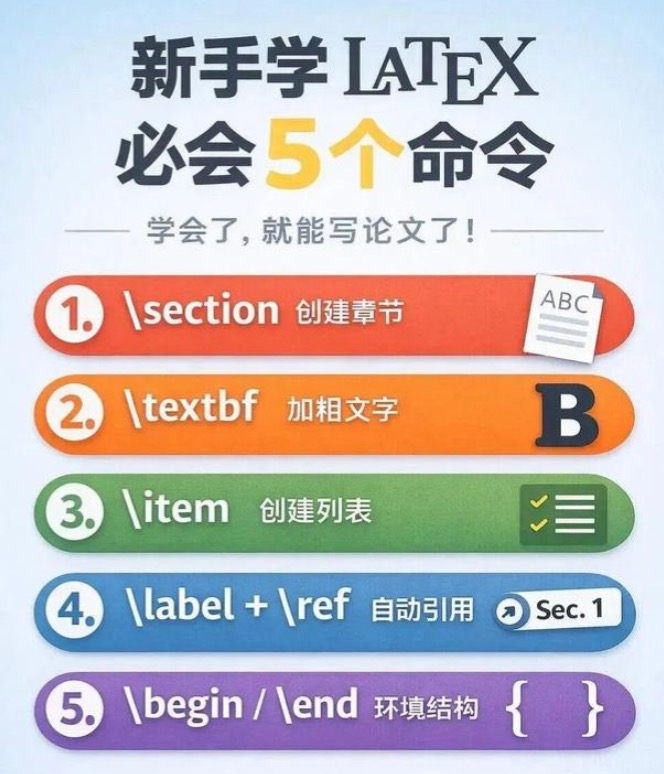
\includegraphics[width=0.5\textwidth]{figures/latex.jpg}
    \caption{LaTeX 文档编译流程示意图}
    \label{fig:latex-process}
\end{figure}